\documentclass[tikz,border=4mm]{standalone}

\usepackage[T1]{fontenc}
\usepackage[scaled=0.92]{helvet}
\renewcommand{\familydefault}{\sfdefault}

\usepackage{graphicx}
\usetikzlibrary{positioning}

\begin{document}

\begin{tikzpicture}
  \node[inner sep=0] (panelA)
    {
\includegraphics[height=9cm]{./panel_a/main.pdf}};
  \node[inner sep=0, right=1.2cm of panelA] (panelB)
    {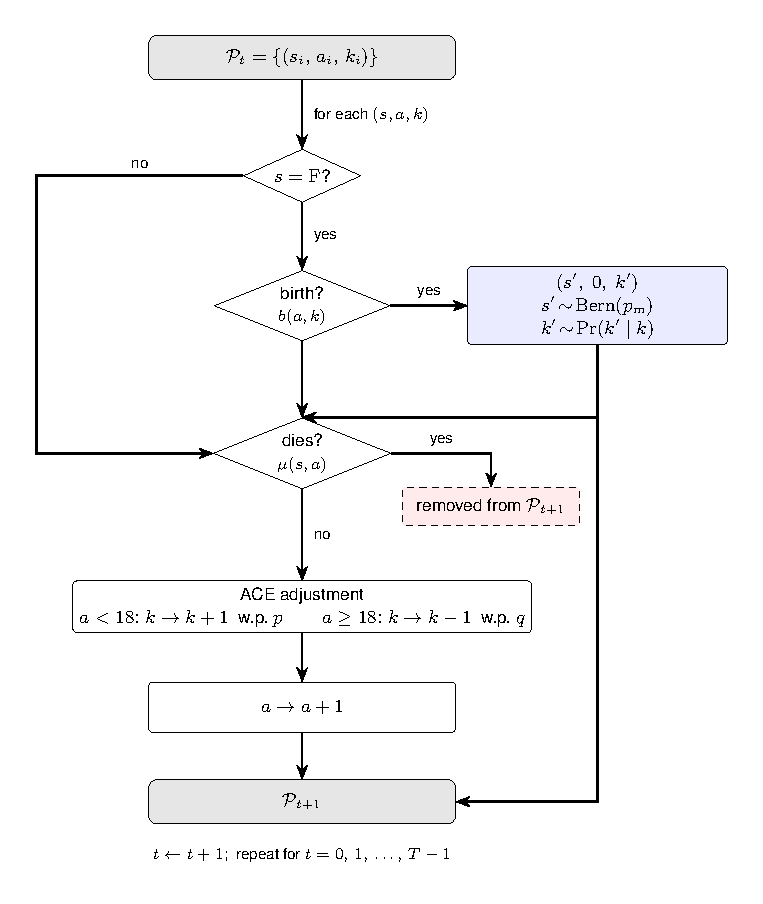
\includegraphics[height=9cm]{./flowchart/main.pdf}};
  \node[above right, font=\small\bfseries] at (panelA.north west) {A};
  \node[above right, font=\small\bfseries] at (panelB.north west) {B};
\end{tikzpicture}

\end{document}
